\section{Линии второго порядка}

\begin{definition}
    \textit{Линиями второго порядка} на плоскоти называются алгебраические линии следующего вида
    \[
    \begin{cases}
        Ax^2 + 2Bxy + Cy^2 + 2Dx + 2Ey + F = 0\\
        A^2 + B^2 + C^2 > 0\\f
    \end{cases}
    \]
\end{definition}
\textbf{В ПДСК:} $\Delta$ = 
$\begin{vmatrix}
    A & B\\
    B & C\\
\end{vmatrix}
$ $-$ неизменная величина при изменении системы координат.\\

\begin{proposition}
    Существует ПДСК, в которой тип кривой второго порядка может быть записан одним из 9 способов (канонических уравнений):
    \begin{itemize}
        \item $\Delta$ > 0 - эллиптический тип
        \begin{enumerate}
            \item $\dfrac{x^2}{a^2}$ + $\dfrac{y^2}{b^2}$ = 1, $a\geq b>0$ $-$ эллипс
            \item $\dfrac{x^2}{a^2}$ + $\dfrac{y^2}{b^2}$ = 0 $-$ пара мнимых пересекающихся прямых
            \item $\dfrac{x^2}{a^2}$ + $\dfrac{y^2}{b^2}$ = -1 $-$ мнимый эллипс
        \end{enumerate}
        \item $\Delta$ < 0 - гиперболический тип
        \begin{enumerate}
            \item $\dfrac{x^2}{a^2}$ - $\dfrac{y^2}{b^2}$ = 1, $a\geq b>0$ $-$ гипербола
            \item $\dfrac{x^2}{a^2}$ - $\dfrac{y^2}{b^2}$ = 0 $-$ пара пересекающихся прямых
        \end{enumerate}
        \item $\Delta$ = 0 - параболический тип
        \begin{enumerate}
            \item $y^2$ = 2px, p > 0 $-$ парабола
            \item $y^2$ = $a^2$, a > 0 $-$ пара параллельных прямых
            \item $y^2$ = 0 $-$ пара совпадающих прямых
            \item $y^2$ = -$a^2$, a > 0 $-$ пара мнимых параллельных прямых
        \end{enumerate}
    \end{itemize}
\end{proposition}

\subsection{Поворот системы координат}

$Ax^2 + 2Bxy + Cy^2 + 2Dx + 2Ey + F = 0$\\

Будем считать, что $B\geq 0$, $A\geq C$. Обнулим коэффициент при ху.\\

Существует угол $\alpha$, на котороый можно повернуть систему координат так, чтобы коэффициент В стал равен 0.
\[
\begin{cases}
    x = cos \alpha \cdot x' - sin \alpha \cdot y'\\
    y = sin \alpha \cdot x' + cos \alpha \cdot y'
\end{cases} \Longrightarrow
\]
\[
A'x'^2 + 2B'x'y' + C'y'^2 + 2D'x' + 2E'y' + F' = 0
\]
\[
A' = A cos^2\alpha + 2B sin \alpha \cdot cos \alpha + C sin^2\alpha
\]
\[
2B' = -2A sin \alpha \cdot cos \alpha + 2B cos^2\alpha - 2B sin^2\alpha + 2C sin \alpha \cdot cos \alpha
\]
\[
C' = A sin^2\alpha - 2B sin \alpha \cdot cos \alpha + C cos^2\alpha\\
\]
При замене координат A' + C' = A + C, $\Delta = \begin{vmatrix}
    A' & B'\\
    B' & C'\\
\end{vmatrix} = \begin{vmatrix}
    A & B\\
    B & C\\
\end{vmatrix}$\\

Покажем, что существует угол $\alpha$ такой что, при повороте системы координат на него, В = 0.
Т.к. $2B' = -2A sin \alpha \cdot cos \alpha + 2B cos^2\alpha - 2B sin^2\alpha + 2C sin \alpha \cdot cos \alpha$
\[
tg \alpha = \dfrac{2B}{A - C}
\]
\begin{enumerate}
    \item Если А = С, то в качестве угла $\alpha$ можно взять угол $\dfrac{\pi}{4}$
    \item Если А $\neq$ C
    \[
    tg^2\alpha + \dfrac{A - C}{B}tg \alpha - 1 = 0 \tab - \text{всегда имеет хотя бы одно решение}
    \]
    $\Longrightarrow$ всегда можно сделать поворот системы координат $\Longrightarrow$
    \[
    \begin{cases}
        B' = 0\\
        A' + C' = A + C\\
        \Delta = const\\
    \end{cases}
    \]
\end{enumerate}

\section{Эллипс}

\begin{wrapfigure}{l}{0.5\textwidth}
    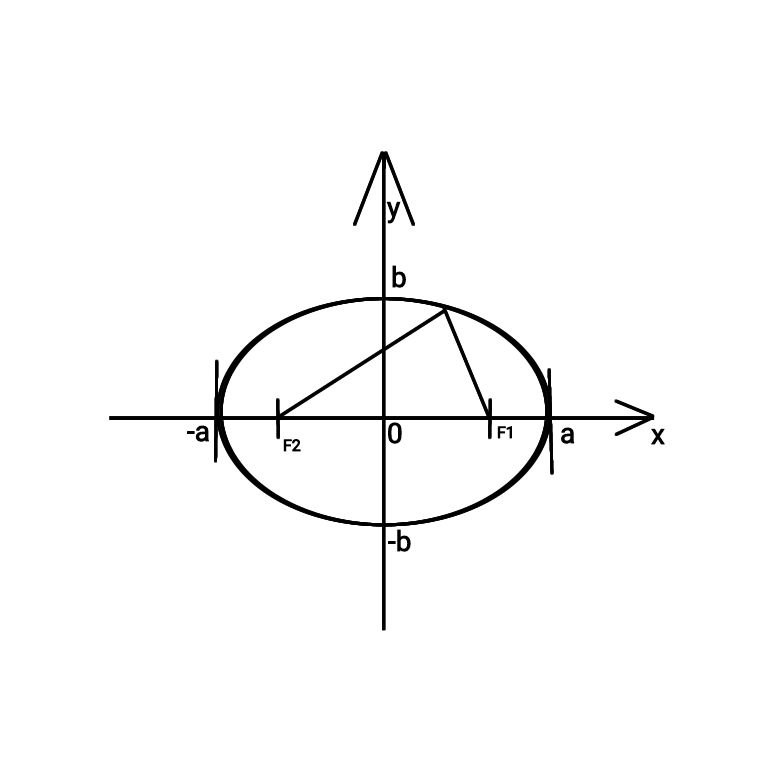
\includegraphics[width=0.84\linewidth]{images/эллипс1.jpeg}
\end{wrapfigure}

\tab\\

Каноническое уравнение эллипса
\[
\dfrac{x^2}{a^2} + \dfrac{y^2}{b^2} = 1, \tab a\geq b > 0
\]

\underline{Свойства множества точек эллипса:}
\begin{enumerate}
    \item Непустое
    \item Ограниченное
    \item Обладает осевой и центральной симметрией
\end{enumerate}

\clearpage
\subsection{Свойства фокусов и эксцентрисетета эллипса}

Рассмотрим a $\neq$ b. Эллипс пересекает оси координат в вершинах эллипса  $-$ $\pm$a, $\pm$b\\
    
Пусть c = $\sqrt{a^2 - b^2}$, тогда фокусы эллипса $-$ точки $F_1$(c, 0), $F_2$(-c, 0).\\
    
Эксцентриситет $\varepsilon$ = $\dfrac{c}{a}$ = $\dfrac{\sqrt{a^2 - b^2}}{a}$, $\varepsilon\in[0, 1)$, причем если $\varepsilon$ = 0, то этот эллипс - окружность.\\

\subsection{Расстояние от точки на эллипсе до фокусов и директрис}

Из теоремы Пифагора
\[
\rho(F_1, A) = (x_0 - c)^2 + y_0^2 = x_0^2 - 2x_0c + c^2 - \dfrac{x_0^2b^2}{a^2} + b^2 = x_0^2 \dfrac{a^2 - b^2}{a^2} - 2x_0\varepsilon a + a^2 = (x_0\varepsilon - a)^2
\]
Аналогично находится $\rho(F_2, A)$, таким образом
\[
\rho(F_1, A) = a - x_0\varepsilon
\]
\[
\rho(F_2, A) = x_0\varepsilon + a
\]

\begin{theorem}
    $\rho(F_1, A)$ + $\rho(F_2, A)$ = 2a
\end{theorem}
\begin{proof}
    $\rho(F_1, A) + \rho(F_2, A)$ = $a - x_0\varepsilon + x_0\varepsilon + a$ = 2a
\end{proof}

\begin{wrapfigure}{l}{0.45\textwidth}
    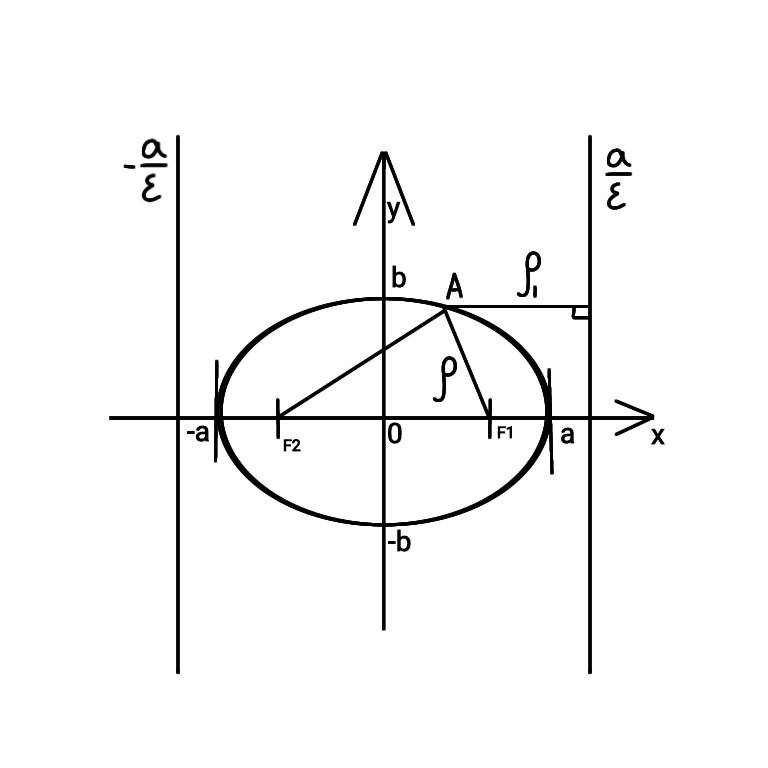
\includegraphics[width=1.0\linewidth]{images/эллипс2.jpeg}
\end{wrapfigure}

\tab\\

\begin{definition}
    Директрисы эллипса задаются уравнением x = $\pm\dfrac{a}{\varepsilon}$
\end{definition}

У окружности директрис $\underline{\text{нет}}$.\\

\begin{proposition}
    Расстояние от точки на эллипсе до фокуса $\rho(F_1, A)$ относится к расстоянию от этой точки до ближайшей директрисы $\rho_1$ как эксцентрисетет.
    \[
    \dfrac{\rho(F_1, A)}{\rho_1} = \varepsilon
    \]
\end{proposition}
\begin{proof}
    Это следует из того, что $\rho(F_1, A) = a - x_0\varepsilon$ и $\rho_1 = \dfrac{a}{\varepsilon} - x_0$
\end{proof}

\clearpage

\subsection{Касательные к эллипсу}

\begin{proposition}
    Пусть эллипс задан уравнением $\dfrac{x^2}{a^2} + \dfrac{y^2}{b^2} = 1$, точка A($x_0$, $y_0$) лежит на эллипсе. Тогда уравнение касательной к эллипсу, проведенной через точку А имеет вид
    \[
    \dfrac{xx_0}{a^2} + \dfrac{yy_0}{b^2} = 1
    \]
\end{proposition}
\begin{proof}
    \begin{enumerate}
        \item Касательные вертикальны $\Longrightarrow$ x = $\pm$a $\longrightarrow$ $x_0$ = $\pm$a, $y_0$ = 0 $\Longrightarrow$ верно.
        \item Касательные не вертикальны $\Longrightarrow$
        \[
        y - y_0 = y'(x_0)(x - x_0)\eqno{(*)}
        \]
        Продифференцируем уравнение эллипса по х:
        \[
        \dfrac{2x}{a^2} + \dfrac{2yy'}{b^2} = 0 \tab\Longrightarrow\tab y'(x_0) = - \dfrac{x_0}{y_0}\cdot\dfrac{b^2}{a^2}
        \]
        Подставим в уравнение (*)
        \[
        y - y_0 = - \dfrac{x_0}{y_0}\cdot\dfrac{b^2}{a^2}\cdot(x - x_0)
        \]
        Домножив на $\dfrac{y_0}{b^2}$, получим
        \[
        \dfrac{x^2}{a^2} + \dfrac{y^2}{b^2} = \dfrac{x_0^2}{a^2} + \dfrac{y_0^2}{b^2} = 1, (\text{т.к точка А лежит на эллипсе)}
        \]
    \end{enumerate}
\end{proof}

\subsection{Оптическое свойство эллипса}
\begin{wrapfigure}{l}{0.45\textwidth}
    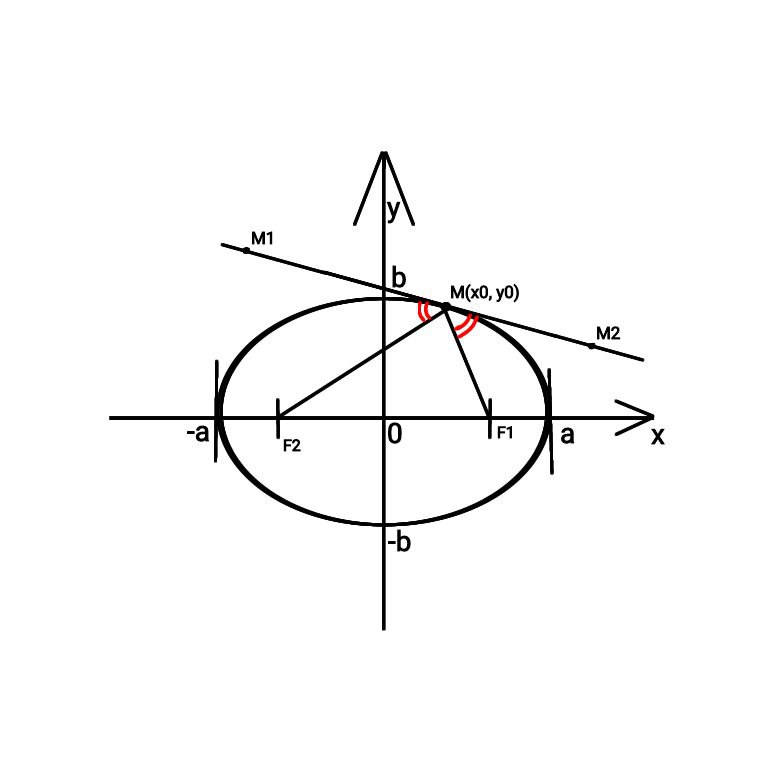
\includegraphics[width=1.0\linewidth]{images/эллипс3.jpeg}
\end{wrapfigure}

\tab\\

\begin{theorem}
    Пусть M($x_0$, $y_0$) - точка на эллипсе, $M_1M_2$ - касательная, проходящая через эту точку. Тогда, углы $F_1MM_2$ и $F_2MM_1$ равны.
\end{theorem}
\begin{proof}
    Достаточно доказать, что
    \[
    \angle(\overline{n}, \overline{F_1M}) = \angle(\overline{n}, \overline{F_2M})
    \]
    \[
    \begin{cases}
        \overline{F_1M}(x_0 + c, y_0)\\
        \overline{F_2M}(x_0 - c, y_0)\\
        \overline{n}(\dfrac{x_0}{a^2}, \dfrac{y_0}{b^2})
    \end{cases} \Longrightarrow
    \]
    \clearpage
    Докажем, что $\dfrac{(\overline{F_1M}, \overline{n})}{|\overline{F_1M}|\cdot|\overline{n}|}$ = $\dfrac{(\overline{F_2M}, \overline{n})}{|\overline{F_2M}|\cdot|\overline{n}|}$
    \[
    \dfrac{(x_0 - c)\dfrac{x_0}{a^2} + \dfrac{y_0^2}{b^2}}{a - \varepsilon x_0} = \dfrac{(x_0 + c)\dfrac{x_0}{a^2} + \dfrac{y_0^2}{b^2}}{a + \varepsilon x_0} \tab\Longrightarrow\tab\text{верно}
    \]
\end{proof}

\section{Гипербола}

\begin{wrapfigure}{l}{0.55\textwidth}
    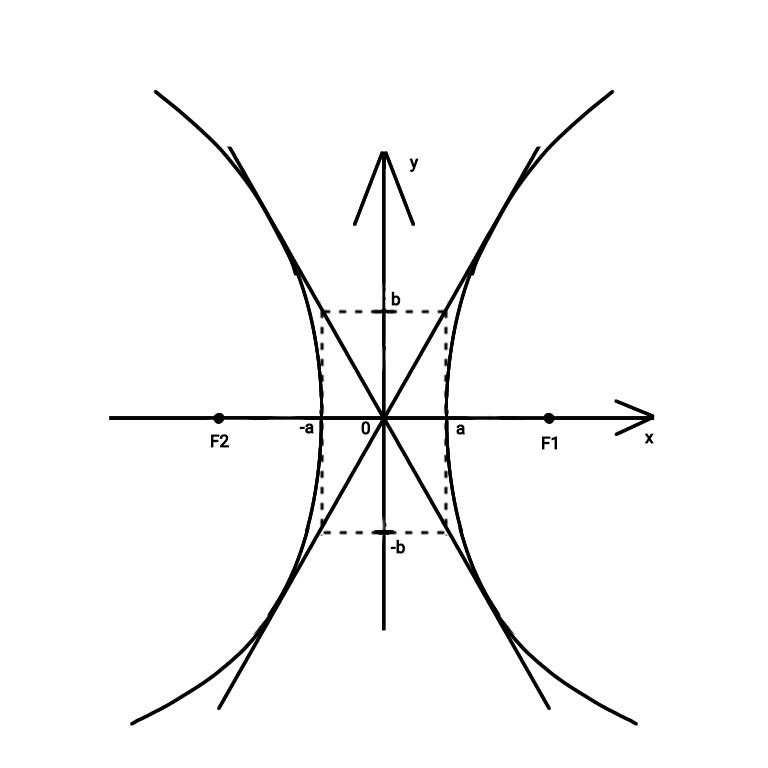
\includegraphics[width=1.0\linewidth]{images/гипербола1.jpeg}
\end{wrapfigure}

\tab\\

Каноническое уравнение гиперболы
\[
\dfrac{x^2}{a^2} - \dfrac{y^2}{b^2} = 1, \tab a, b \neq 0
\]

\underline{Свойства множества точек гиперболы:}
\begin{enumerate}
    \item Непустое
    \item Неограниченное
    \item Обладает осевой и центральной симметрией
\end{enumerate}

\tab\\ \tab\\ \tab\\ \tab\\ \tab\\ \tab\\ \tab\\ \tab\\ \tab\\

\subsection{Свойства фокусов и эксцентрисетета гиперболы}

Из уравнения гиперболы y = $\pm\dfrac{b}{a}\sqrt{x^2 - a^2}$.\\

Пусть x > 0, тогда y = $\dfrac{b}{a}\sqrt{x^2 - a^2}$ $\Longrightarrow$ множество точек гиперболы находится ниже прямой y = $\dfrac{b}{a}x$. Аналогично при x < 0 множество точек гиперболы находится ниже прямой y = -$\dfrac{b}{a}x$.\\

Пусть c = $\sqrt{a^2 + b^2}$, тогда фокусы эллипса $-$ точки $F_1$(c, 0), $F_2$(-c, 0).\\
    
Эксцентриситет $\varepsilon$ = $\dfrac{c}{a}$ = $\dfrac{\sqrt{a^2 + b^2}}{a}$, $\varepsilon > 1$.\\

\subsection{Расстояние от точки на гиперболе до фокусов и директрис}

\begin{wrapfigure}{l}{0.6\textwidth}
    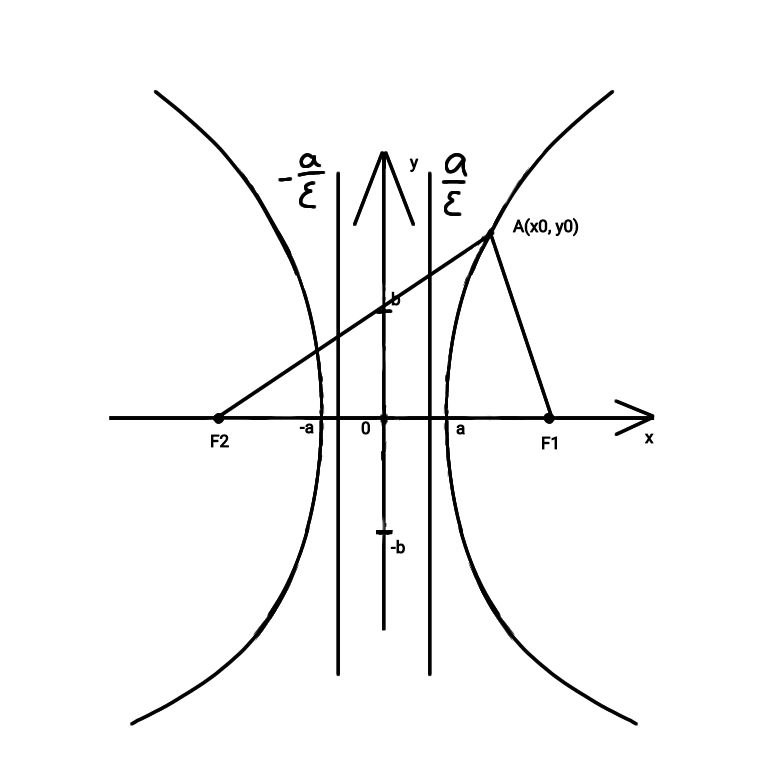
\includegraphics[width=0.8\linewidth]{images/гипербола2.jpeg}
\end{wrapfigure}

\tab\\

Пусть А($x_0$, $y_0)$ - точка на гиперболе. Тогда расстояния от нее до фокусов равны

\[
\rho(F_1, A) = |a - \varepsilon x_0|
\tab\\
\rho(F_2, A) = |a + \varepsilon x_0|
\]

Знак, с которым раскрываются модули, зависит от того, на какой ветви гиперболы находится точка А
\begin{enumerate}
    \item x > 0 $\Longrightarrow$
    $\begin{cases}
        \rho(F_1, A) = \varepsilon x_0 - a\\
        \rho(F_2, A) = a + \varepsilon x_0
    \end{cases}$
    \item x < 0 $\Longrightarrow$
    $\begin{cases}
        \rho(F_1, A) = a - \varepsilon x_0\\
        \rho(F_2, A) = -a - \varepsilon x_0
    \end{cases}$
\end{enumerate}

\begin{proposition}
    $|\rho(F_1, A)$ - $\rho(F_2, A)|$ = 2a
\end{proposition}
\tab\\
\begin{definition}
    Директрисы гиперболы задаются уравнением x = $\pm\dfrac{a}{\varepsilon}$
\end{definition}

\begin{proposition}
    Расстояние от точки на гиперболе до фокуса $\rho(F_1, A)$ относится к расстоянию от этой точки до ближайшей директрисы $\rho_1$ как эксцентрисетет.
    \[
    \dfrac{\rho(F_1, A)}{\rho_1} = \varepsilon
    \]
\end{proposition}
\clearpage

\subsection{Касательные к гиперболе}

Пусть гипербола задана уравнением $\dfrac{x^2}{a^2} - \dfrac{y^2}{b^2} = 1$, точка A($x_0$, $y_0$) лежит на гиперболе. Тогда уравнение касательной к гиперболе, проведенной через точку А имеет вид
    \[
    \dfrac{xx_0}{a^2} - \dfrac{yy_0}{b^2} = 1
    \]
\subsection{Оптическое свойство гиперболы}

\begin{wrapfigure}{l}{0.55\textwidth}
    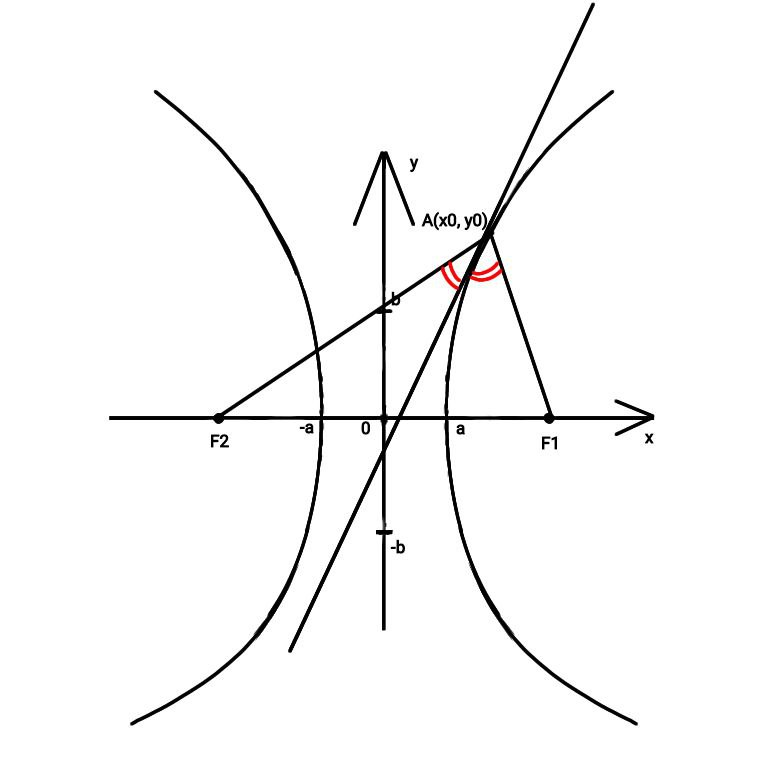
\includegraphics[width=.8\linewidth]{images/гипербола3.jpeg}
\end{wrapfigure}
\tab\\ 
\begin{theorem}
    Пусть A($x_0$, $y_0$) - точка на гиперболе, через которую провели касательную. Тогда, углы, образованные этой касательной и фокальными радиусами точки, равны.
\end{theorem}
\tab\\ \tab\\ \tab\\ \tab\\ \tab\\ \tab\\ \tab\\ \tab\\ \tab\\ 
\section{Парабола}

\begin{wrapfigure}{l}{0.6\textwidth}
    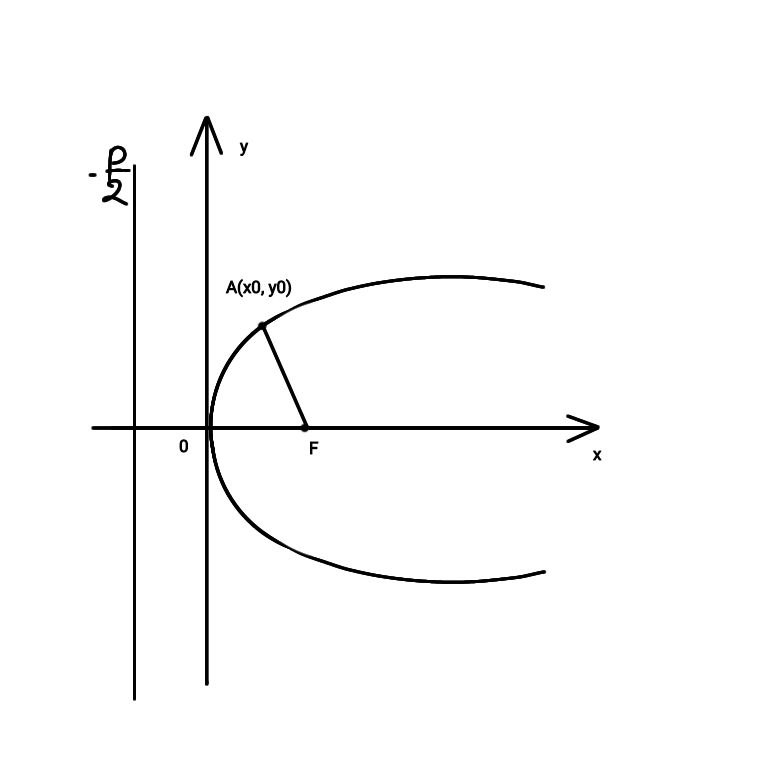
\includegraphics[width=.8\linewidth]{images/парабола1.jpeg}
\end{wrapfigure}

\tab\\ 

Каноническое уравнение параболы
\[
y^2 = 2px, p > 0
\]

\underline{Свойства множества точек эллипса:}
\begin{enumerate}
    \item Непустое
    \item Неограниченное
    \item Симметричное относительно одной из осей
\end{enumerate}
\clearpage

\subsection{Свойства фокуса и эксцентрисетета параболы}

Эксцентрисетет параболы равен 1, фокус один и находится в точке с координатами ($\dfrac{p}{2}$, 0).

\subsection{Расстояние от точки на параболы до фокуса и директрисы}

Пусть А($x_0$, $y_0)$ - точка на параболе. Тогда расстояние от нее до фокуса равно

\[
\rho(F, A) = x_0 + \dfrac{p}{2}
\]

\begin{definition}
    Директриса параболы задается уравнением x = -$\dfrac{p}{2}$
\end{definition}

Расстояние от точки А($x_0$, $y_0)$ на параболе до директрисы равно $x_0 + \dfrac{p}{2}$

\subsection{Касательные к параболе}

Пусть парабола задана уравнением $y^2 = 2px$, точка A($x_0$, $y_0$) лежит на параболе. Тогда уравнение касательной к параболе, проведенной через точку А имеет вид
    \[
    yy_0 = p(x + x_0)
    \]
    
\subsection{Оптическое свойство параболы}

\begin{wrapfigure}{l}{0.5\textwidth}
    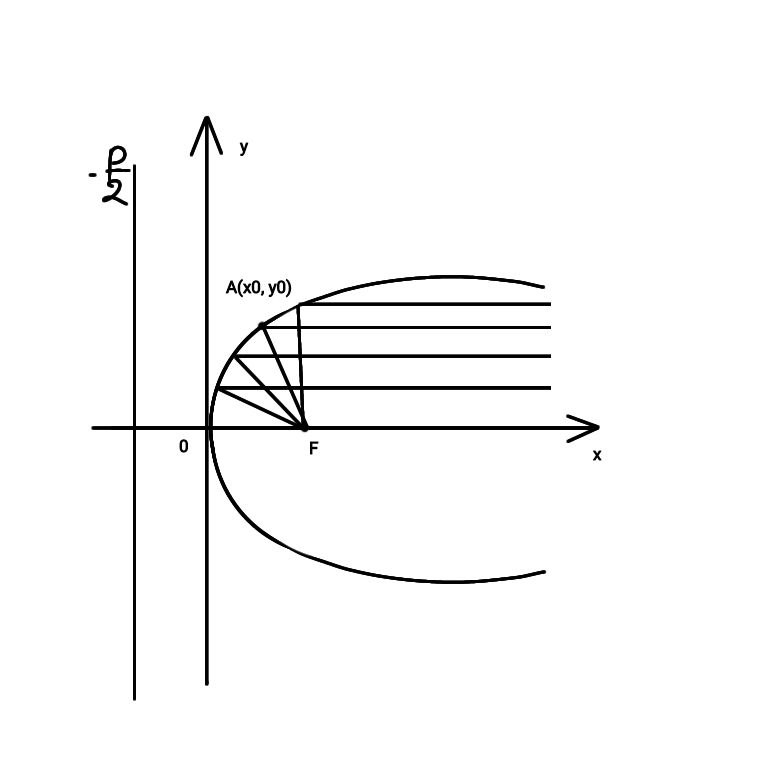
\includegraphics[width=1.0\linewidth]{images/парабола2.jpeg}
\end{wrapfigure}

\tab\\
\begin{theorem}
    Параллельные лучи приходят в фокус параболы и проходят одинаковые расстояния.
\end{theorem}
